\documentclass[11pt, oneside]{article} 
\usepackage{geometry}
\geometry{letterpaper} 
\usepackage{graphicx}
	
\usepackage{amssymb}
\usepackage{amsmath}
\usepackage{parskip}
\usepackage{color}
\usepackage{hyperref}

\graphicspath{{/Users/telliott_admin/Dropbox/Tex/png/}}
% \begin{center} 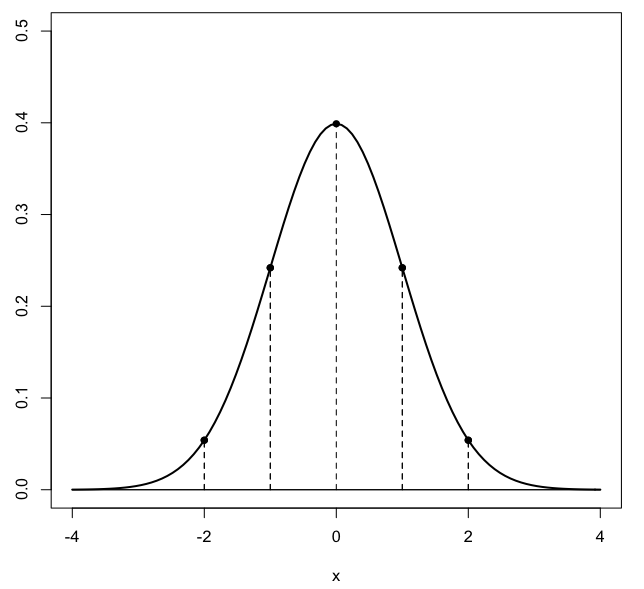
\includegraphics [scale=0.4] {gauss3.png} \end{center}

\title{Code}
\date{}

\begin{document}
\maketitle
\Large
Once we get to$2^5$, let alone GF($2^8$), it becomes pretty tedious to calculate by hand.

Here is my version of the mod function, set up to work on decimals.  The variable mod is the irreducible polynomial.  For $2^8$ that would be $100011011$ which is decimal $256 + 27 = 283$.  The exp would be $8$ in this case.

\begin{verbatim}
def nspaces(n):
    b = len(bin(mod))
    return len(bin(n)) - b
    
def modulus(n,exp,mod):
    while True:
        if n < 2**exp:
            return n
        n = n ^ (mod << nspaces(n))
\end{verbatim}

What we're doing is taking bin(283) which is \textbf{0b100011011} as a Python string, and then getting the length of that string (which includes the "0b" part, but we leave both here and below on bin(n)).

In the loop, the default value of base is 8 and $2^8 = 256$. If we've already cleared all the high bits, or there were none, just return $n$.  Otherwise $bin(n)$ is at least as large as $b$, so we promote mod by left-shifting it out the correct amount, and then do XOR with that result and $n$.

The other part is the multiplication.

\begin{verbatim}
def multiply(a,b,exp,mod):
    # binary string, reversed
    s = bin(b)[2:][::-1]
    n = 0
    for c in s:
        if c == '1':
            n = n ^ a
        a = a << 1
    return modulus(n,exp,mod)
\end{verbatim}

In this function we get the binary digits of the second multiplicand (removing the extra "0b"), and then consume those binary digits one by one.  At each stage, if the digit is "1", then XOR $a$ with the accumulator.  And at the end, promote $a$ by left-shift.  It takes some time to work something like this out.

\subsection*{note}

Actually, if you know some Python, you might take a look at the copy of math.py that is in this project.  To make calling the functions either, I wrote a wrapper around multiply that returns the multiply function.  Thus it "knows" the exp and mod values which are passed into the wrapper.  

multiply can be called without supplying exp and mod, but these values can be changed to try different exponents.

\subsection*{text}

I test it by reproducing the powers of \textbf{0x03} from a reference.  My version of the table looks like this in hex.  I actually prefer to work with ints, but the reference has hex, so here it is.

\begin{verbatim}
01 03 05 0f 11 33 55 ff 1a 2e 72 96 a1 f8 13 35
5f e1 38 48 d8 73 95 a4 f7 02 06 0a 1e 22 66 aa
e5 34 5c e4 37 59 eb 26 6a be d9 70 90 ab e6 31
53 f5 04 0c 14 3c 44 cc 4f d1 68 b8 d3 6e b2 cd
4c d4 67 a9 e0 3b 4d d7 62 a6 f1 08 18 28 78 88
83 9e b9 d0 6b bd dc 7f 81 98 b3 ce 49 db 76 9a
b5 c4 57 f9 10 30 50 f0 0b 1d 27 69 bb d6 61 a3
fe 19 2b 7d 87 92 ad ec 2f 71 93 ae e9 20 60 a0
fb 16 3a 4e d2 6d b7 c2 5d e7 32 56 fa 15 3f 41
c3 5e e2 3d 47 c9 40 c0 5b ed 2c 74 9c bf da 75
9f ba d5 64 ac ef 2a 7e 82 9d bc df 7a 8e 89 80
9b b6 c1 58 e8 23 65 af ea 25 6f b1 c8 43 c5 54
fc 1f 21 63 a5 f4 07 09 1b 2d 77 99 b0 cb 46 ca
45 cf 4a de 79 8b 86 91 a8 e3 3e 42 c6 51 f3 0e
12 36 5a ee 29 7b 8d 8c 8f 8a 85 94 a7 f2 0d 17
39 4b dd 7c 84 97 a2 fd 1c 24 6c b4 c7 52 f6 01
\end{verbatim}

We won't exercise this a great deal here (see the markdown pages for that).

But it's nice to have it set up so that we can specify the base and the irreducible polynomial.  Recall that we generated the powers of \textbf{0x02} for GF($2^4$):

\begin{verbatim}
> python gmath.py 3
01 03 05 04 07 02 06 01
> python gmath.py 4
01 02 04 08 09 0b 0f 07
0e 05 0a 0d 03 06 0c 01
> python gmath.py 5
01 02 04 08 10 05 0a 14
0d 1a 11 07 0e 1c 1d 1f
1b 13 03 06 0c 18 15 0f
1e 19 17 0b 16 09 12 01
>>>> 
\end{verbatim}

which matches what we had before in decimal.

Here is code that checks all the multiplicative inverses in GF($2^4$), which we also saw previously.

\begin{verbatim}
>>> from gmath import multiplier
>>> f = multiplier(exp=4,mod=25)
>>> for i in range(1,16):
...     for j in range(1,16):
...         if f(i,j) == 1:
...             print i,j
... 
1 1
2 12
3 8
4 6
5 15
6 4
7 14
8 3
9 13
10 11
11 10
12 2
13 9
14 7
15 5
>>>
\end{verbatim}

With a few quick changes, it runs just as fast for GF($2^8$).

\subsection*{GF($2^5$)}

I obtained an irreducible polynomial for this field from

\url{http://mathworld.wolfram.com/IrreduciblePolynomial.html}

\[ x^5 + x^2 + 1 = 100101 = 37 \]

\begin{verbatim}
> python gmath.py 5
  1   2   4   8  16   5  10  20
 13  26  17   7  14  28  29  31
 27  19   3   6  12  24  21  15
 30  25  23  11  22   9  18   1
>
\end{verbatim}

I just guessed that \textbf{0x02} would work as a generator, and it appears that it does.

\end{document}